In this section we face the case in which the demand curves are unknown and can be subject to abrupt changes. More precisely, our proposed simulator present an abrupt change every 100 days involving the demand curves for each product for each customer.
We use different approaches to face the same problem:
\begin{itemize}
    \item UCB-1 algorithm with abrupt change detection.
    \item UCB-1 algorithm with sliding window.
\end{itemize}
\subsection{Abrupt change detection}
\label{learner2}
In this case, at the end of each day, the learner, before updating its arms, checks either the conversion rate has changed or not for each product for each price. The naivest way is to compute the conversion rate of the current day $\alpha_t(p, a)$ for product $p$ given price $a$ and compare it with the average of the conversion rates of the last days $\hat{\alpha}_{t-1}(p, a)$.\\ We set a threshold $\delta$ such that if :
\begin{align*}
        \alpha_t(p, a) \not\in \left[ \hat{\alpha}_{t-1}(p, a) - \delta, \hat{\alpha}_{t-1}(p, a) + \delta \right]
\end{align*}
then that specific conversion rate has just changed. Due to the high noise that characterizes the realizations of the environment it is incredibly hard to understand why a realization might be out of the range.
\\In order to overcome this issue we propose a slightly advanced approach: instead of comparing the last conversion rate with the average of the last conversion rates, we say that the conversion rate for a specific product for a given price has changed if:
\begin{align*}
    \hat{\alpha}_{t, t -\lambda}(p, a) \not\in \left[ \hat{\alpha}_{t-\lambda, 1}(p, a) - \delta, \hat{\alpha}_{t-\lambda, 1}(p, a) + \delta \right]
\end{align*}
where $\hat{\alpha}_{t, t -\lambda}(p, a)$ is the average of the last $\lambda$ conversion rates, whereas $ \hat{\alpha}_{t-\lambda, 1}(p, a)$ is the average of the first $t - \lambda$ conversion rates for that product $p$ at price $a$. This method reveals to be more robust to the noise of the environment, but requires more days to detect an anomaly, nevertheless, we can achieve great results setting $\lambda$ to 5 as we can see from Figures ~\ref{fig:reward61}, \ref{fig:regret61}, \ref{fig:cum_reg61}.\\
Once a conversion rate has been spotted as changing, all the data related to that specific pair (price, arm) are dropped, since those data are no more relevant.\\
Here the code for the detection algorithm:
\begin{minted}[breaklines]{python}
    def change_detection_test(self, pulled_arm, report):
        conv_rate = report.get_conversion_rate()
        for product, arm in enumerate(pulled_arm):
            delta = 0.3
            mean1, mean2 = 0, 0

            if len(self.conv_rate_history[product][arm]) > 10:
                last_conv_rates = self.conv_rate_history[product][arm][-self.splitter:]
                last_conv_rates.append(conv_rate[product])

                mean1 = np.mean(self.conv_rate_history[product][arm][:-self.splitter])

                mean2 = np.mean(last_conv_rates)

            if self.t_arms[product, arm] > 11 and (mean1 < mean2 - delta or mean1 > mean2 + delta) and not np.isinf(
                    self.upper_bounds[product, arm]):
                # detected an abrupt change
                self.t_arms[product, arm] = 0
                self.means[product, arm] = 0
                self.upper_bounds[product, arm] = np.inf
                self.seen[product, arm] = 0
                self.conv_rate_history[product][arm] = [conv_rate[product]]
\end{minted}
\subsection{Insights on abrupt change detection algorithm}
\label{learner1}
Now we want to investigate and understand if under the assumption to already know all the conversion rates will change, we can improve the performance of the learner: when a change for a single pair (price, product) is detected, all the conversion rates are dropped. From Figures~\ref{fig:reward62}, \ref{fig:regret62}, \ref{fig:cum_reg62} we notice the two algorithms have comparable performances, thus, there is no reason to use a more specific algorithm as the one just introduced.

\subsection{Sliding window}
Finally we change the UCB-1 algorithm implementing the sliding window to keep track of the most relevant samples.
The main idea behind this algorithm is the demand curves are currently smoothly changing, thus samples loose importance with the time.\\
In order to avoid old samples to affect the learner's performance, we use a sliding window of size $\sigma$: in other words we compute the estimated conversion rates and their upper bounds using only the last $\sigma$ samples.\\
The drawback of sliding window is the learner has a short memory about the past, thus, if it is used on a stationary environment, it it will be outperformed by a stationary UCB-1 algorithm, since it will behave in a more exploratory way.
Using a sliding window of size 50, we can see from Figures~\ref{fig:reward63}, \ref{fig:regret63}, \ref{fig:cum_reg63}, the learner with the change detection algorithm outperforms
the one using the sliding window. This should not surprise us for the following reasons:
\begin{itemize}
    \item Our environment is characterized by three stationary phases. When a change occurs, it is abrupt instead of being smooth: sliding window has been thought to face the second scenario, thus it will be slower to converge.
    \item For the first 100 days, the environment is stationary, thus the sliding window struggle to converge since it is discarding the oldest samples, despite they are still useful.
\end{itemize}




\subsection{Results}
In this subsection we present the experimental results got interacting with a non stationary environment for 300 days and the number of daily customers is drawn every day from a Normal distribution $\mathcal{N}(300, 10)$.
\begin{figure}[ht]
    \begin{center}
    \includegraphics[width=0.6\textwidth]{img/rewards_active2.png}
    \caption{Change detection UCB Reward}
    \label{fig:reward61}
    \end{center}
\end{figure}
\begin{multicols}{2}
    \begin{figure}[H]
        \begin{center}
        \includegraphics[width=0.5\textwidth]{img/regret_active2.png}
        \caption{Change detection UCB Regret}
        \label{fig:regret61}
        \end{center}
    \end{figure}
    \columnbreak
    \begin{figure}[H]
        \begin{center}
        \includegraphics[width=0.5\textwidth]{img/cumulative_regret_active2.png}
        \caption{Change detection UCB Cumulative regret}
        \label{fig:cum_reg61}
        \end{center}
    \end{figure}
\end{multicols}

\begin{figure}[ht]
    \begin{center}
    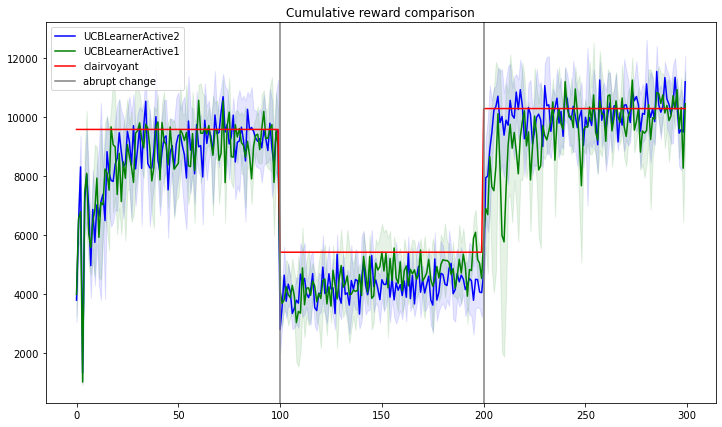
\includegraphics[width=0.6\textwidth]{img/reward_LA1vsLA2.png}
    \caption{Reward comparison between Learner 1 (algorithm in Subsection~\ref{learner1}) and Learner 2 (algorithm in Subsection~\ref{learner2})}
    \label{fig:reward62}
    \end{center}
\end{figure}
\begin{multicols}{2}
    \begin{figure}[H]
        \begin{center}
        \includegraphics[width=0.5\textwidth]{img/regret_LA1vsLA2.png}
        \caption{Regret comparison between Learner 1 (algorithm in Subsection~\ref{learner1}) and Learner 2 (algorithm in Subsection~\ref{learner2})}
        \label{fig:regret62}
        \end{center}
    \end{figure}
    \columnbreak
    \begin{figure}[H]
        \begin{center}
        \includegraphics[width=0.5\textwidth]{img/cumulative_regret_LA1vsLA2.png}
        \caption{Cumulative regret comparison between Learner 1 (algorithm in Subsection~\ref{learner1}) and Learner 2 (algorithm in Subsection~\ref{learner2})}
        \label{fig:cum_reg62}
        \end{center}
    \end{figure}
\end{multicols}


\begin{figure}[ht]
    \begin{center}
    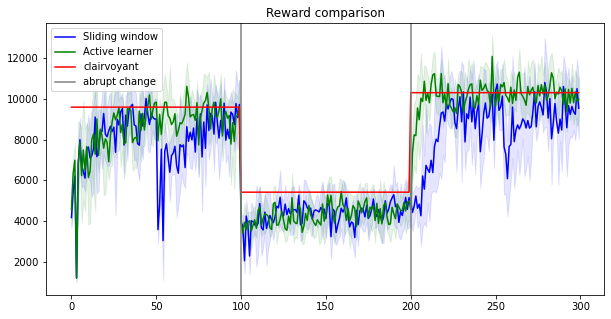
\includegraphics[width=0.6\textwidth]{img/sw_vs_active_reward.png}
    \caption{TODO: CAMBIARE IMMAGINI Reward comparison between Learner with change detection algorithm and Learner with sliding window}
    \label{fig:reward63}
    \end{center}
\end{figure}
\begin{multicols}{2}
    \begin{figure}[H]
        \begin{center}
        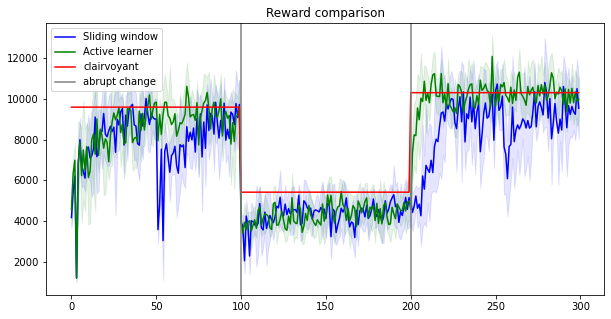
\includegraphics[width=0.5\textwidth]{img/sw_vs_active_reward.png}
        \caption{Regret comparison between Learner with change detection algorithm and Learner with sliding window}
        \label{fig:regret63}
        \end{center}
    \end{figure}
    \columnbreak
    \begin{figure}[H]
        \begin{center}
        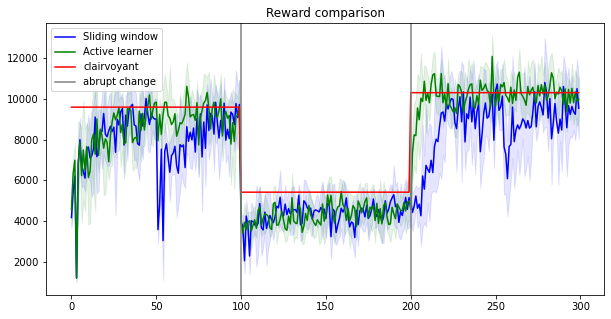
\includegraphics[width=0.5\textwidth]{img/sw_vs_active_reward.png}
        \caption{Cumulative regret comparison between Learner with change detection algorithm and Learner with sliding window}
        \label{fig:cum_reg63}
        \end{center}
    \end{figure}
\end{multicols}

